\capitolo{Controlli Automatici}
Ripasso di controlli automatici con focus su: Trasformata di Laplace; Diagrammi di Bode; Sistemi del secondo ordine; Luogo delle radici; Criteri di stabilità; Analisi di sistemi nel tempo e in frequenza.

\sezione{Trasformata di Laplace}
La trasformata di Laplace bilatera del segnale $x:\mathbb{R} \rightarrow \mathbb{C}$ è la funzione $X:\mathbb{C} \rightarrow \mathbb{C}$, $s \rightarrow X(s) := \int^\infty_{-\infty} x(t)e^{-st} dt $, per ogni $s=\sigma + j\omega\in \mathbb{C}$ per cui l'integrale converge. Si denota come $\laplace{x(t)} = X(s)$.

\sottosezione{Proprietà}
Principali proprietà della trasformata di Laplace.
\begin{itemize}
    \item Traslazione in t: $\laplace{x(t+\beta)} = e^{s\beta}X(s)$
    \item Traslazione in s: $\laplace{e^{s_0t}x(t)} = X(s-s_0)$
    \item Cambio di scala: $\laplace{x(at)} = \frac{1}{\abs{a}}X(\frac{s}{a})$
    \item Derivata in s: $\laplace{tx(t)}=-\derivata{X(s)}{s}$
    \item Convoluzione: $\laplace{v(t)*w(t)} = V(s)W(s)$
    \item Integrazione in t: $\laplace{\int^t_{-\infty} x(\tau) d\tau }=\frac{X(s)}{s}$
    \item Antritrasformata di Laplace: $x(t)=\frac{1}{2\pi} \int^\infty_{-\infty}X(\sigma+j\omega) e^{(\sigma+j\omega)t} d\omega$
    \item Derivata in t: $\laplace{\derivata{x(t)}{t}} = s X(s)$
\end{itemize}

%% valutare di copiarne altre da appunti di controlli

\sottosezione{Funzione di Trasferimento}
Per un sistema LTI, la funzione di trasferimento \(H(s)\) è definita come il rapporto della trasformata di Laplace dell'uscita \(Y(s)\) e dell'ingresso \(X(s)\) del sistema, assumendo condizioni iniziali nulle:
\(H(s)=\frac{Y(s)}{X(s)}\).

\sezione{Diagrammi di Bode}
Per rappresentare le risposte armoniche si utilizza una coppia di diagrammi detti di Bode:
\begin{enumerate}
    \item $\abs{G(j\omega)}$ funzione di $\omega$
    \item $\arg{G(j\omega)}$ funzione di $\omega$
\end{enumerate}

Sono diagrammi semilogaritmici (anche logaritmici) utili per rappresentare ampi intervalli di pulsazioni e quindi permettono di osservare facilmente amplificazioni e attenuazioni.

\sottosottosezione{Decibel}
Il decibel, adimensionale perché indica rapporti di grandezze equivalenti dimensionalmente, è definito per le ampiezze come $G_{dB} = 20\log_{10}{\abs{H(j\omega)}}$. Il decibel è usato nei diagrammi di Bode per rappresentare le ampiezze delle risposte in esame.

\sottosottosezione{Fasi}
Le fasi $\arg{1+j\omega \tau}=\arctan{\omega \tau}$, 

\sottosottosezione{Regole di tracciamento}
Nel caso di ampiezze:
\begin{enumerate}
    \item Costanti: rette orizzontali
    \item Poli: Per ogni ordine n hanno pendenza di $-n\cdot 20dB$ per decade 
    \item Zeri: Per ogni ordine n hanno pendenza di $+n\cdot 20dB$ per decade
\end{enumerate}

Nel caso di fasi:
\begin{enumerate}
    \item Costanti: $0 rd$
    \item Poli: Per ogni ordine n hanno pendenza di $-n\cdot \frac{\pi}{4}$ per decade, per una durata totale di due decadi
    \item Zeri: Per ogni ordine n hanno pendenza di $n\cdot \frac{\pi}{4}$ per decade, per una durata totale di due decadi
\end{enumerate}

\sezione{Sistemi del Secondo Ordine} \label{sistemi_ordine_2}
I sistemi del secondo ordine si definiscono come \(G(s)=\frac{K \omega_n^2}{s^2+2\xi\omega_n s +\omega_n^2}\), dove \(\omega_n\) è la frequenza naturale dei poli e  \(\xi\) è il fattore di smorzamento. Ha per radici 
\(s_{1,2}=-\xi \omega_n \pm \omega_n\sqrt{\xi^2-1}\), dove: per \(\xi < 1\) i due poli sono complessi coniugati; per \(\xi = 1\) i due poli sono coincidenti; per \(\xi > 1\) i due poli sono reali distinti.

\sottosezione{Risposta al gradino}
Parametri tipici della risposta al gradino sono: 
\begin{itemize}
    \item \(t_\text{rise}\), tempo di salita, definito come il tempo impiegato per passare dal \(10\%\) al \(90\%\) del valore finale\footnote{Tuttavia permette di sapere solo ciò che accade negli istanti iniziali. Un sistema con un buon tempo di risposta potrebbe divergere e non avremmo modo di rendencene conto guardando solo questo tempo.}; \item \(M_p\) massima sovraelongazione come incremento, in percentuale, sul valore finale; 
    \item \(t_\text{settling}\), tempo di assestamento, definito come il tempo per arrivare e permanere all'interno di una certa banda entro l'\(1\%\) del valore finale.
\end{itemize}

\sottosezione{Effetto dello smorzamento}
Lo smorzamento interviene in diverso modo sulla dinamica di un sistema in base al valore che assume. In particolare vengono distinte tre regioni:
\begin{enumerate}
    \item \(\xi > 1\) sistema sovrasmorzato, non presenta oscillazioni o sovraelongazione
    \item \(\xi = 1\) sistema criticamente smorzato, è quanto più veloce il sistema può rispondere in assenza di oscillazioni
    \item \(\xi < 1\) sistema sottosmorzato, presenta oscillazioni e sovraelongazione
\end{enumerate}

\paragrafo{Massima sovraelongazione:}
La massima sovraelongazione in un sistema del secondo ordine dipende unicamente dal valore dello smorzamento. Un valore che va tenuto a mente è \(\xi \simeq 0.7\) per cui si ottiene \(M_p = 5\%\).

\begin{figure}[h]
    \centering
    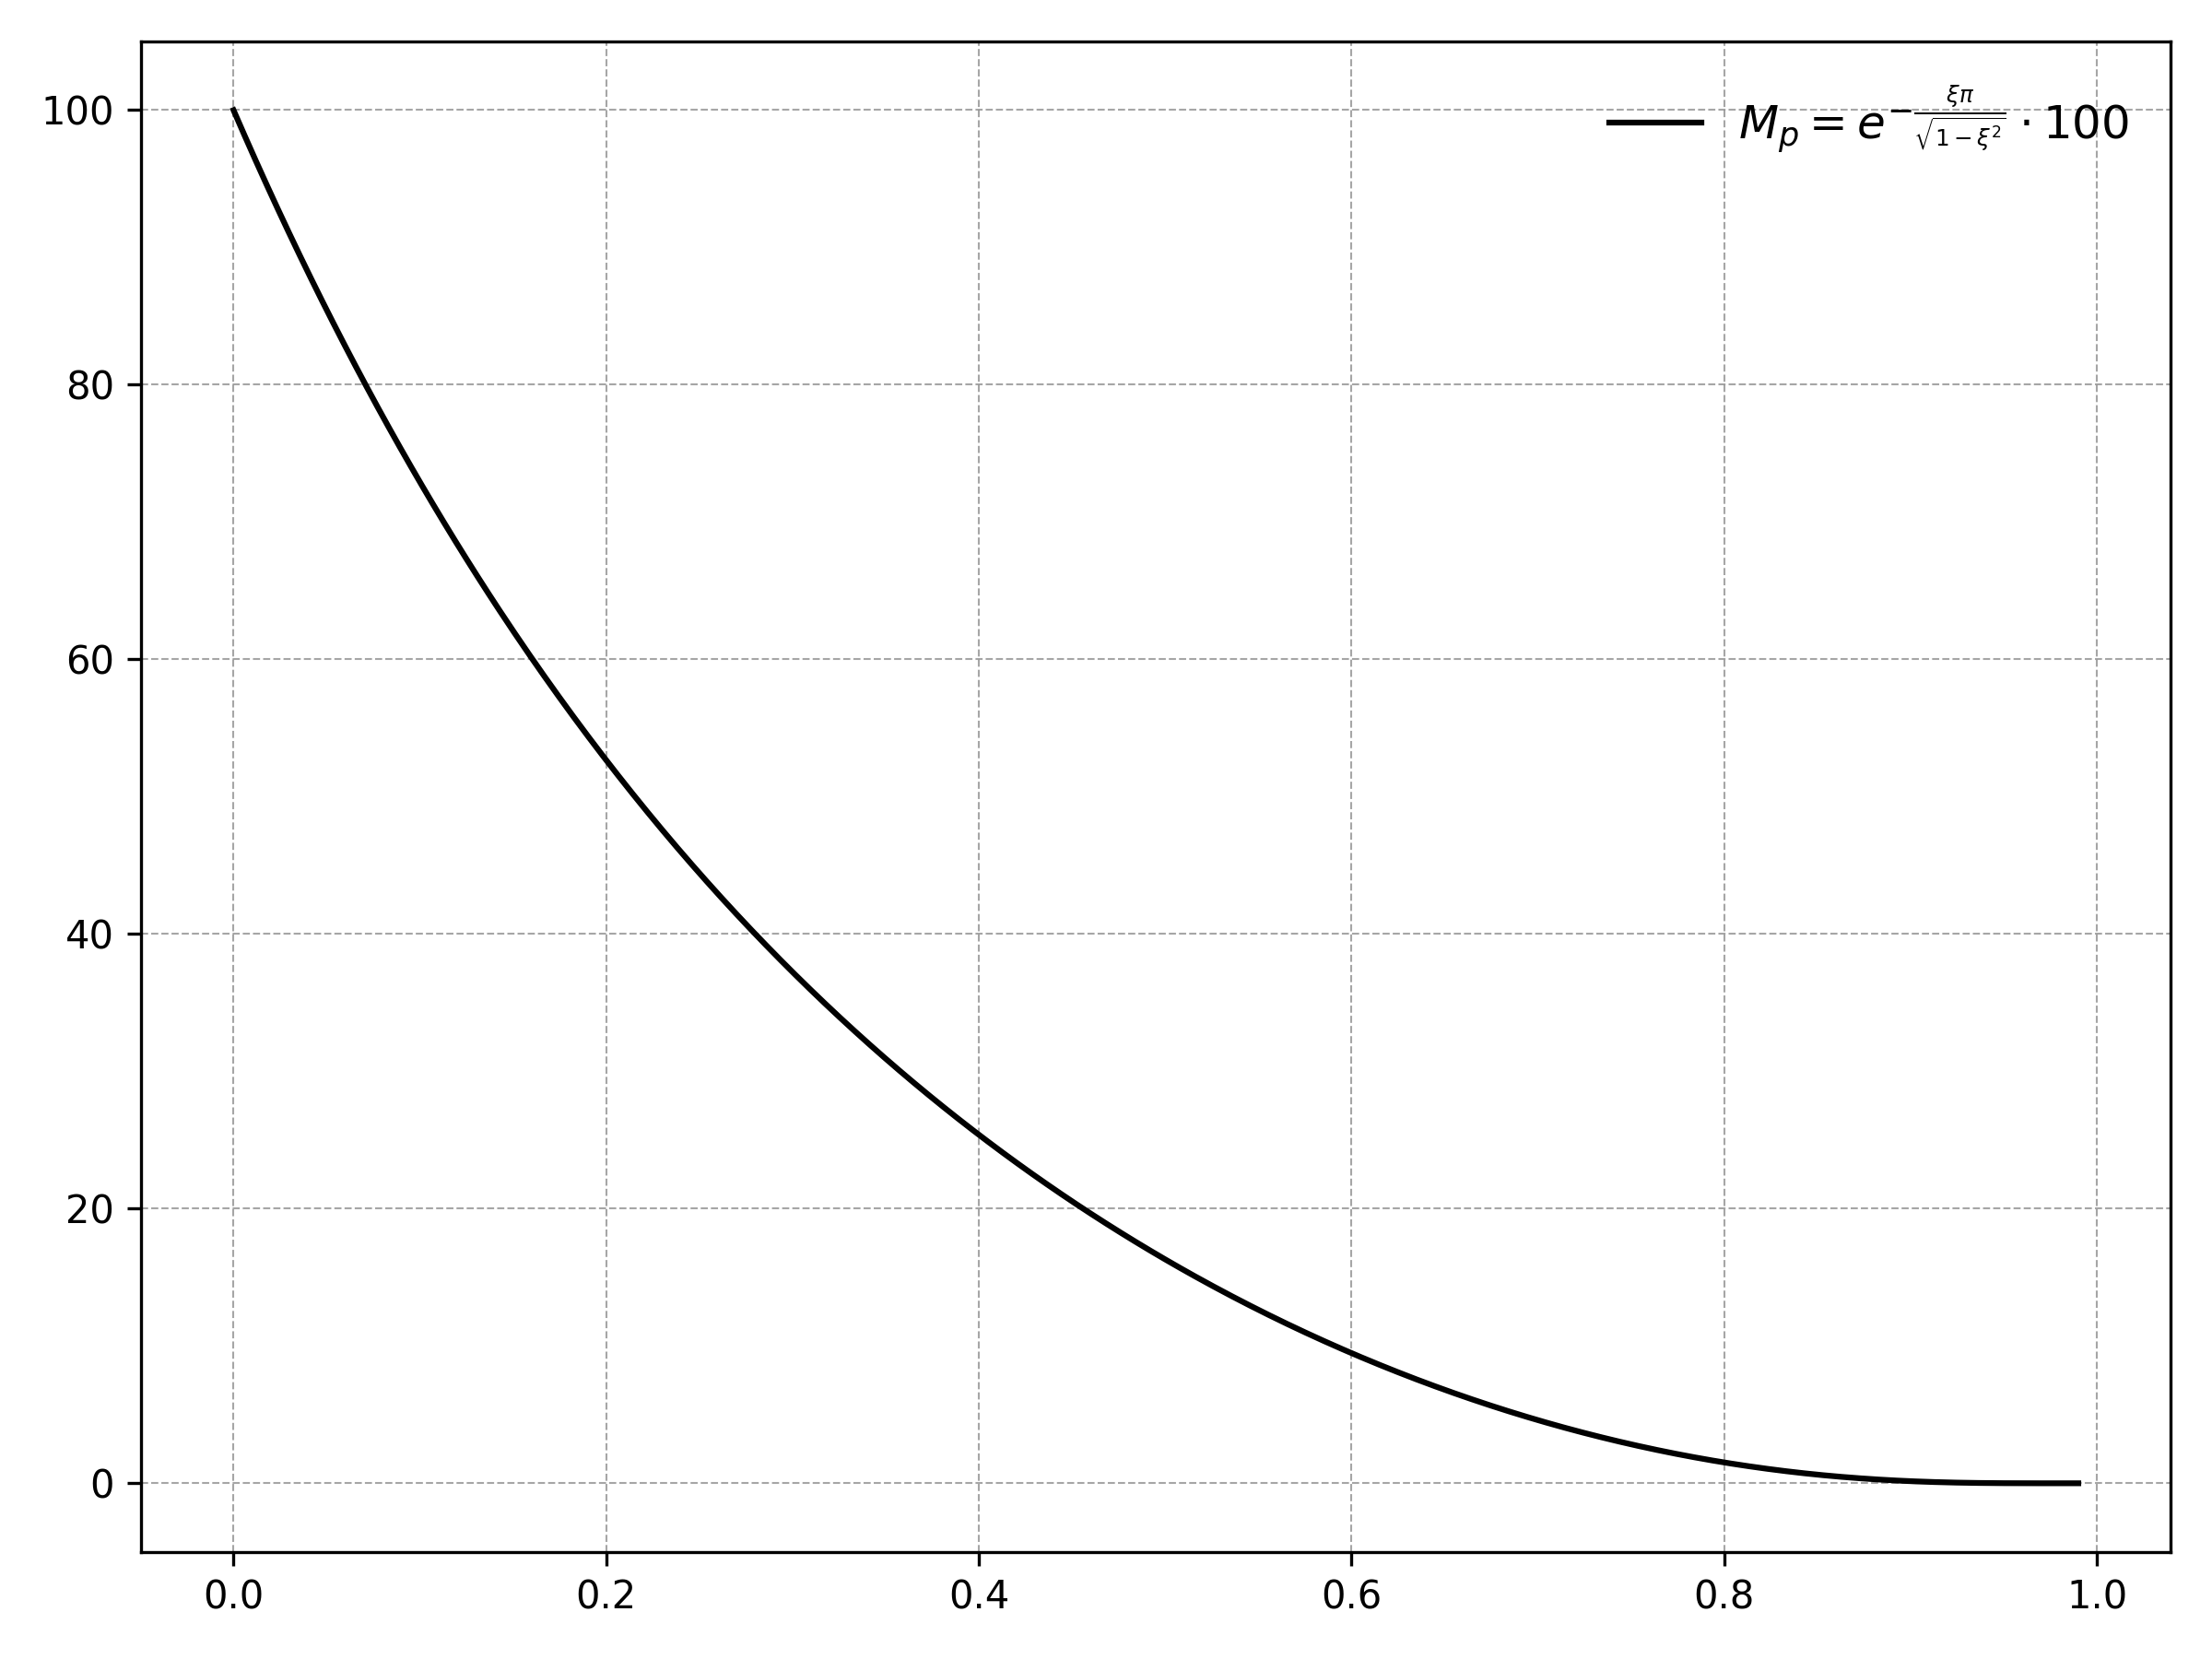
\includegraphics[width=0.4\textwidth]{Immagini/sovraelongazione_xi.png}
    \caption{Influenza del fattore di smorzamento nella sovraelongazione}
\end{figure}

\paragrafo{Tempo di assestamento:}
Nei libri, solitamente, è presente una relazione del tipo \(t_s \propto \frac{1}{\xi \omega_n} \), tuttavia non tiene conto della non monotonia di \(t_s\) al variare di \(\xi\).
In particolare, risulta più corretto:
\[
\begin{cases}
    t_s \propto \frac{1}{\omega_n} \text{ \ } \downarrow \text{\ se \ } \uparrow \omega_n \\
    \propto \frac{1}{\xi} \text{\ fino 0.7, oltre 0.7 \ } \propto \xi
\end{cases}
\]
In questo modo risulta chiaro come convenga operare per pulsazioni naturali alte, e per sovraelongazioni \(\xi \in [0.6;1.1]\) {\color{red}{Come mai in questo range, cosa significa?}}

\sezione{Luogo delle radici}
Strumento che consente di valutare graficamente l'andamento delle radici del denominatore di una funzione di trasferimento ottenuta mettendo in retroazione il blocco di andata costituito da $G(s)$ e blocco proporzionale $K$, e il blocco di retroazione $1$. 
Definito $G(s)=\frac{N(s)}{D(s)}$, monico e coprimo; il polinomio caratteristico del sistema in retroazione unitaria è dato da $D(s) + K N(s) = 0$, e rappresenta i poli di $W(s)=\frac{K N(s)}{D(s) + K N(s)}$. Al variare di $K$, con il luogo delle radici, è possibile analizzare la posizione dei poli del sistema a catena chiusa $W(s)$.

\sottosezione{Step}
\begin{enumerate}[label=\roman*.]
    \item Funzione di trasferimento del sistema ad anello aperto: Scrivere la funzione di trasferimento del sistema ad anello aperto $G(s)H(s)$, dove: $G(s)H(s)=N(s)D(s)$; $N(s)$: numeratore del sistema; $D(s)$: denominatore del sistema. Questa funzione è solitamente espressa in termini di poli e zeri del sistema.

    \item Trovare i poli e gli zeri: Determinare i poli (tali che $D(s)=0$) e gli zeri (tali che $N(s)=0$) del sistema ad anello aperto. I poli (disegnati solitamente con una "x") determinano le posizioni iniziali delle traiettorie del luogo delle radici, mentre gli zeri (disegnati solitamente con un "o") ne determinano le destinazioni finali.

    \item Determinare la quantità di traiettorie: Il numero di rami (traiettorie del luogo delle radici) è uguale al numero di poli del sistema ad anello aperto. Ogni ramo inizia da un polo del sistema e tende verso uno zero del sistema, o verso l'infinito se ci sono più poli che zeri.

    \item Trovare l'asse reale coinvolto nel luogo delle radici: Determinare i tratti dell'asse reale che fanno parte del luogo delle radici. Un segmento sull'asse reale fa parte del luogo delle radici se alla sua destra ci sono un numero dispari di poli e zeri.

    \item Determinare i punti di separazione e arrivo (Asintoti): Se ci sono più poli che zeri, calcolare gli asintoti delle traiettorie del luogo delle radici, che indicano dove i rami tendono all'infinito. Gli asintoti possono essere trovati con: $\textup{Angoli degli asintoti}=\frac{(2k+1)\pi}{n-m}$
    Dove $n$ è il numero di poli, $m$ è il numero di zeri; $k=0,1,2,…$, di cui devono essere indagati tutti i valori fino a quando non si giunga ad una ripetizione degli angoli. 
    Il punto di intersezione con l'asse reale è dato da: $\sigma_a=\frac{\sum \textup{Poli}-\sum \textup{Zeri}}{n-m}$

    \item Trovare i punti di rottura (breakaway) sull'asse reale: Se due o più rami si uniscono o si separano sull'asse reale, questo avviene in punti detti punti di rottura. Per determinare tali punti, risolvere la derivata della funzione caratteristica del sistema: $\derivata{​(1+KG(s)H(s))}{s}=0$, o in modo empirico calcolando \( \sum^m_1\frac{1}{\sigma - z_i} = \sum^n_1 \frac{1}{\sigma-p_i} \) dove \( z_i \) è lo zero e \( p_i \) il polo, questo restituisce la coordinata sull'asse reale del punto studiato.

    \item Calcolare gli angoli di partenza e arrivo: Determinare l'angolo di partenza per i rami che si staccano dai poli complessi e l'angolo di arrivo per quelli che si avvicinano agli zeri complessi. Questi angoli sono calcolati con le equazioni basate sulla posizione relativa di poli e zeri complessi rispetto al polo o allo zero in questione.

    \item Determinare i punti di intersezione con l'asse immaginario (criterio di Routh-Hurwitz): Verificare se i rami del luogo delle radici attraversano l'asse immaginario. Questo può essere fatto utilizzando il criterio di Routh-Hurwitz per trovare i valori di \( K \) per cui il sistema ha poli con parte reale nulla (ossia poli puramente immaginari).

    \item Tracciare il luogo delle radici: Con tutte le informazioni raccolte, tracciare il diagramma del luogo delle radici:
    \begin{enumerate}
        \item Parti dai poli ad anello aperto.
        \item Disegna i rami lungo l'asse reale e seguendo gli asintoti.
        \item Mostra come i rami si avvicinano agli zeri o tendono all'infinito.
        \item Indica chiaramente i punti di rottura, intersezioni con l'asse immaginario e altri dettagli chiave.
    \end{enumerate}
\end{enumerate}

\sottosezione{Proprietà extra}
\begin{itemize}
    \item Per trovare un punto nel luogo della radici, noti gli angoli tra ciascuno zero e quel punto \( \theta_z \), e tra angoli tra ciascun polo e quel punto \( \theta_p \): \( \sum \theta_z - \sum \theta_p = -180° \).
    \item Lo smorzamento nel diagramma corrisponde a un angolo \( \theta = \cos^{-1} (\psi) \).
    \item Sussiste una relazione tra il guadagno ad anello aperto e \( K_\text{tot} = \frac{1}{\abs{G_\text{open}H}} = \frac{\Pi L_{p,i}}{\Pi L_{z,i}} \) con \( L_p \) e \( L_z \) lunghezze dei poli/zeri, ossia distanza tra polo/zero e punto di interesse. Se non ci sono poli o zeri, vanno posti a 1.
\end{itemize}

\sottosezione{Esempio}
Per esempio fare il luogo delle radici di $G(s) = \frac{s + 3}{(s + 1)(s + 5)(s + 10)}$ risulta nel seguente grafico:
\begin{figure}[h]
    \centering
    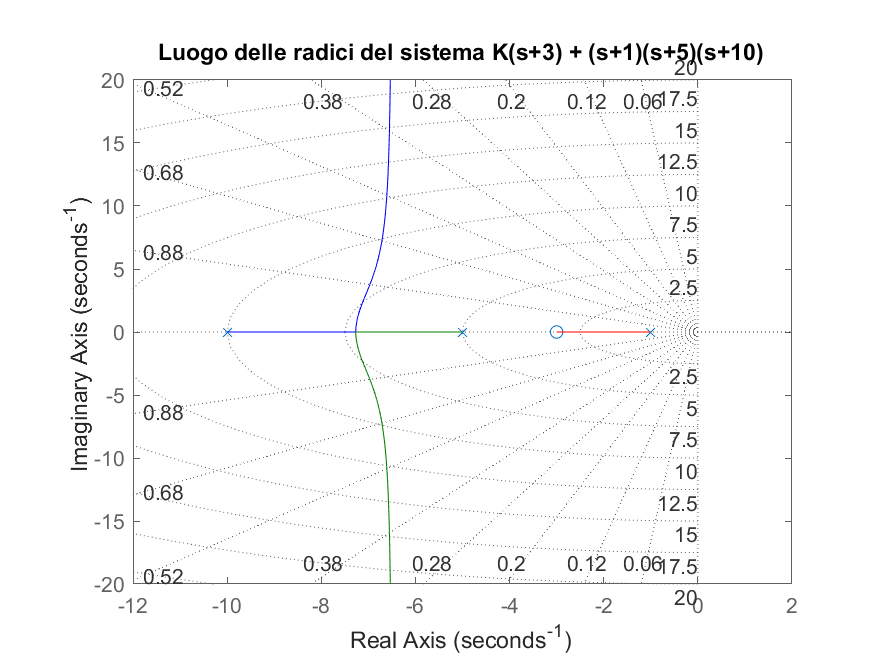
\includegraphics[width=0.4\textwidth]{Immagini/luogo_delle_radici.png}
\end{figure}

%% Rivedere parte su luogo delle radici


\sezione{Criteri di Stabilità}
Per lo studio dei sistemi è importante conoscerne la stabilità, ossia se il sistema reagisce in modo controllato ad un dato ingresso.
Ci sono diversi tipi di criteri di stabilità alcuni sono grafici, altri analitici.

\sottosezione{Criterio Stabilità BIBO}
Con stabilità BIBO si intende che il sistema abbia una risposta limitata ad un ingresso limitato. Nota bene, questa stabilità non implica stabilità asintotica.

\sottosezione{Criterio di Stabilità dei Poli della funzione di trasferimento}
In un sistema lineare rappresentato da una funzione di trasferimento \(H(s)=\frac{N(s)}{D(s)}\) con \(N(s)\) e \(D(s)\) coprimi, la stabilità dipende dalla posizione dei poli. Questo criterio è necessario ma non sufficiente.

\begin{itemize}
    \item Per un sistema causale e stabile, tutti i poli devono avere una parte reale negativa, cioè devono trovarsi nel semipiano sinistro del piano complesso \(\mathbb{R}(s)<0\).
    \item Se anche un solo polo ha una parte reale positiva \(\mathbb{R}(s)>0\), il sistema è instabile.
    \item Se i poli si trovano sulla linea immaginaria pura \(\mathbb{R}(s)=0\), il sistema è marginalmente stabile, cioè risponderà con oscillazioni permanenti e costanti.
\end{itemize}


\sottosezione{Criterio di Routh-Hurwitz}
Il criterio di Routh-Hurwitz permette di verificare la stabilità di un sistema senza calcolare esplicitamente i poli della funzione di trasferimento. Si basa sullo sviluppo di una tabella chiamata tabella di Routh:

Supposto di avere un polinomio caratteristico \(P(s)=a_n s^n+a_{n-1}s^{n-1}+⋯+a_1 s+a_0\) con \(a_n,a_{n-1},…,a_0\) coefficienti reali. La tabella di Routh si costruisce come segue:

\begin{itemize}
    \item Prima riga: Inserisci i coefficienti degli elementi di grado pari, a partire da \(a_n\)
    \item Seconda riga: Inserisci i coefficienti degli elementi di grado dispari, partendo da \(a_{n-1}\)
    \item Righe successive: Gli elementi delle righe successive si calcolano utilizzando i coefficienti delle righe precedenti. Ogni elemento della riga \(i+2\) si calcola con la formula: \(R_{i+2,j} =\frac{ R_{i,1} R_{i+1,j+1} - R_{i+1,1} R_{i,j+1}}{R_{i+1,1}}\)
    dove \(R_{i,j}\) rappresenta l'elemento nella riga \(i\) e colonna \(j\) della tabella.
    \item Continua a costruire la tabella fino ad avere una riga per ogni grado di \(s\) (fino a \(s^0\)).
\end{itemize}

\paragrafo{Condizione di Stabilità:}

Il criterio di Routh-Hurwitz stabilisce che il sistema è stabile se e solo se tutti i termini della prima colonna della tabella di Routh hanno lo stesso segno (positivi o negativi).
Ogni cambio di segno nella prima colonna corrisponde a un polo con parte reale positiva, quindi a un segno di instabilità.

\sottosezione{Criterio di Bode}\label{CriterioBode}
Per il criterio di Bode, può essere analizzata la stabilità di un sistema tramite due parametri principali, il margine di fase \(m_\phi\) e il margine di guadagno \(m_a\). 

\begin{center}
Un sistema è stabile se \(m_\phi>0,m_a>0\).
\end{center}

\begin{enumerate}
    \item \textbf{Margine di fase:} la differenza in gradi tra la fase del sistema e \(-180^\circ\) alla frequenza di attraversamento del guadagno unitario (o nullo in dB) \(\omega_a\): \(m_\phi=\pi\angle{L(j\omega_a)}\). Indica quanto ritardo in fase il sistema può sopportare prima di diventare instabile. 
    \item \textbf{Margine di guadagno:} il rapporto di guadagno necessario per portare il sistema ad attraversare il punto critico, ossia per \(\omega_\pi\) tc \(\angle{L(j\omega_a)}=-\pi\): \(m_a=\frac{1}{\abs{L(j\omega_\pi)}}=-\abs{L(j\omega_\pi)}_{dB}\). Indica l'incremento in termini di guadagno che un elemento del sistema può sopportare prima di diventare instabile. 
\end{enumerate}

\sottosezione{Criterio di Nyquist}
Il criterio di Nyquist è un metodo grafico utilizzato per analizzare la stabilità dei sistemi con retroazione (feedback) attraverso un'analisi della risposta in frequenza.
Il criterio di Nyquist si applica tipicamente ai sistemi descritti dalla funzione di trasferimento ad anello aperto \(L(s)\), data dal prodotto del guadagno dell'impianto \(G(s)\) e del guadagno del controllore \(H(s)\), \(L(s)=G(s)H(s)\).

\sottosottosezione{Diagramma di Nyquist}
Per applicare il criterio, si costruisce il diagramma di Nyquist, ovvero la curva tracciata nel piano complesso \(\mathbb{C}\) dalla funzione \(L(i\omega)\) al variare della frequenza \(\omega\) da 0 a \(+\infty\) (e poi da \(+\infty\) a \(-\infty\), se necessario). Questa curva rappresenta la risposta in frequenza del sistema in catena aperta, con la parte reale di \(L(i\omega)\) sull'asse x e la parte immaginaria sull'asse y.

\sottosottosezione{Stabilità}
Per determinare la stabilità del sistema a ciclo chiuso, il criterio di Nyquist si basa su un'analisi del numero di avvolgimenti del diagramma di Nyquist attorno al punto -1 nel piano complesso. Questo punto rappresenta la condizione critica in cui la retroazione positiva (instabilità) potrebbe prevalere, rendendo instabile il sistema a ciclo chiuso.

Numero di avvolgimenti: Conta il numero di volte che il diagramma di Nyquist avvolge il punto -1 nel piano complesso, considerando il senso di rotazione.

Relazione con i poli instabili: Per la stabilità a ciclo chiuso, il numero di avvolgimenti attorno a -1 deve essere tale da compensare eventuali poli a parte reale positiva nel sistema a ciclo aperto.

Il criterio di Nyquist afferma che il numero di avvolgimenti netti N della curva di Nyquist attorno al punto -1 (contati in senso antiorario come positivi e in senso orario come negativi) deve soddisfare la relazione \(N=P-Z\), dove: 
\begin{itemize}
    \item N è il numero di avvolgimenti netti del diagramma attorno al punto -1
    \item P è il numero di poli a ciclo aperto di \(L(s)\) nel semipiano destro (ovvero i poli a parte reale positiva, che renderebbero instabile il sistema a ciclo chiuso)
    \item Z è il numero di zeri a ciclo chiuso di \(1+L(s)\) nel semipiano destro (equivalente al numero di poli instabili del sistema a ciclo chiuso)
\end{itemize}
Per garantire la stabilità del sistema a ciclo chiuso, il numero Z deve essere zero, ossia non ci devono essere poli a ciclo chiuso con parte reale positiva.

Sistema stabile: Se il sistema a ciclo aperto non ha poli a parte reale positiva \(P=0\), allora la stabilità a ciclo chiuso è garantita se il diagramma di Nyquist non avvolge il punto -1.
Sistema con poli instabili: Se il sistema a ciclo aperto ha poli a parte reale positiva \(P>0\), allora il diagramma di Nyquist deve avvolgere il punto -1 un numero di volte pari a P per garantire la stabilità a ciclo chiuso.